\documentclass[9pt,twocolumn,twoside,]{pnas-new}

%% Some pieces required from the pandoc template
\providecommand{\tightlist}{%
  \setlength{\itemsep}{0pt}\setlength{\parskip}{0pt}}

% Use the lineno option to display guide line numbers if required.
% Note that the use of elements such as single-column equations
% may affect the guide line number alignment.

%%
%%


%%
%%

\usepackage[T1]{fontenc}
\usepackage[utf8]{inputenc}

% Pandoc citation processing
\newlength{\csllabelwidth}
\setlength{\csllabelwidth}{3em}
\newlength{\cslhangindent}
\setlength{\cslhangindent}{1.5em}
% for Pandoc 2.8 to 2.10.1
\newenvironment{cslreferences}%
  {}%
  {\par}
% For Pandoc 2.11+
\newenvironment{CSLReferences}[3] % #1 hanging-ident, #2 entry spacing
 {% don't indent paragraphs
  \setlength{\parindent}{0pt}
  % turn on hanging indent if param 1 is 1
  \ifodd #1 \everypar{\setlength{\hangindent}{\cslhangindent}}\ignorespaces\fi
  % set entry spacing
  \ifnum #2 > 0
  \setlength{\parskip}{#2\baselineskip}
  \fi
 }%
 {}
\usepackage{calc} % for calculating minipage widths
\newcommand{\CSLBlock}[1]{#1\hfill\break}
\newcommand{\CSLLeftMargin}[1]{\parbox[t]{\csllabelwidth}{#1}}
\newcommand{\CSLRightInline}[1]{\parbox[t]{\linewidth - \csllabelwidth}{#1}}
\newcommand{\CSLIndent}[1]{\hspace{\cslhangindent}#1}


\templatetype{pnasresearcharticle}  % Choose template

\title{On the Emergence of Culturally Constructed Landscapes}

\author[a]{Jonathan S Reeves}
\author[a]{Tomos Proffitt}
\author[a]{Lydia Luncz}

  \affil[a]{Max Planck Institute for Evolutionary Anthropology,
Technological Primate Research Group, Deutscher Platz 6., Leipzig,
Germany, 04103}


% Please give the surname of the lead author for the running footer
\leadauthor{Reeves}

% Please add here a significance statement to explain the relevance of your work
\significancestatement{While primate behavioral ecological studies are
argued to provide novel insight about hominin evolution, placing these
insights within a broader evolutionary context is difficult. Our model
demonstrates how agent-based modeling can be used to elucidate broader
environment-tool use dynamics that may have been relevant to the
evolution of tool use within the hominin lineage.}


\authorcontributions{Please provide details of author contributions
here.}

\authordeclaration{There are no conflicts of interest.}


\correspondingauthor{\textsuperscript{2} E-mail:
\href{mailto:jonathan_reeves@eva.mpg.de}{\nolinkurl{jonathan\_reeves@eva.mpg.de}}}

% Keywords are not mandatory, but authors are strongly encouraged to provide them. If provided, please include two to five keywords, separated by the pipe symbol, e.g:
 \keywords{  Tool Transport |  Niche Construction |  Percussive
tools |  Primate Archaeology |  Agent-Based Modeling  } 

\begin{abstract}
Primates and humans represent two end members on the spectrum of tool
using behaviors. On the primate side, while tool use provides access to
otherwise inaccessible resources, opportunities for it are largely
constrained by the distribution of resources and tool materials. On the
other hand, tool use among humans represents the access to novel
resources but a capacity to advantageously modify the surrounding
environment on an unprecedented scale. Despite the assumed role of tools
in shaping the evolutionary trajectory of the hominin clade, how the
comparatively simple tool using behaviors observed in non-human primates
became such a transformative trait in humans remains unclear. While
behavioral ecological studies of chimpanzee tool use provide a window of
insight into the root of tool use in the hominin lineage, placing these
behaviors within a broader evolutionary context requires both linking
these small scale behaviors are related to processes that operate on
broader spatio-temporal scales as well as to a static archaeological
record. Here we present an agent-based model that elucidates the long
term dynamics between small-scale tool use, the environment, and the
formation of the archaeological record. In doing so, we are able to show
that while primate tool use is largely constrained by environmental
parameters, there are circumstances in which such behaviors can
positively modify their environments over the long term. While our
results also suggest that these processes leave tangible corollaries in
the archaeological record, they are variable and may be difficult to
link back to the behaviors that produced them.
\end{abstract}

\dates{This manuscript was compiled on \today}
\doi{\url{www.pnas.org/cgi/doi/10.1073/pnas.XXXXXXXXXX}}

\begin{document}

% Optional adjustment to line up main text (after abstract) of first page with line numbers, when using both lineno and twocolumn options.
% You should only change this length when you've finalised the article contents.
\verticaladjustment{-2pt}

\maketitle
\thispagestyle{firststyle}
\ifthenelse{\boolean{shortarticle}}{\ifthenelse{\boolean{singlecolumn}}{\abscontentformatted}{\abscontent}}{}

% If your first paragraph (i.e. with the \dropcap) contains a list environment (quote, quotation, theorem, definition, enumerate, itemize...), the line after the list may have some extra indentation. If this is the case, add \parshape=0 to the end of the list environment.

\acknow{We thank the Max Planck Institute for supporting this research.}

The adaptive success of humans is largely based on our ability to use
tools to mitigate or modify whatever environmental circumstances that
confront us. Over human evolutionary history, this trait has facilitated
the expansion of humans and their ancestors across every environment in
the terrestrial world (1). While it is now understood that the emergence
of this trait is the result of feedback between genetic, ecological, and
cultural processes over time (2--9), the mechanisms that transformed
this behavior from the simple forms of tool use that are observed across
multiple taxa to an obligate reliance on material culture remains
unclear. Primate behavioral ecology provides a potential window of
insight into the origin of this trait as primate tool use is argued to
approximate the types of tool using behaviors present at the root of the
hominid lineage (10--13). Thus, examining the dynamic ecological
settings in which tool-use occurs allows researchers to generate
hypotheses of how complex tool use emerged and was maintained in the
hominin lineage (14). However, placing primate tool use within a broader
evolutionary context requires (1) understanding its relationship within
broader long term environmental dynamics and (2) establishing
corollaries linking these dynamics to the variation in a recoverable
material record (15, 16).

For example, nut-cracking among chimpanzees is largely constrained by
the environment. Nevertheless, some groups are argued to move stone
tools potentially kilometers from where they are naturally found (17,
18). This slow redistribution of stone may influence the number of
opportunities for tool use across a given landscape 10s of years. In
addition, the location of nut-trees, which control the availability of
nuts, change due to the death of old trees and growth of new ones over
centuries. Therefore, understanding the relationship between small scale
tool transport behaviors, the broader environment, and its effect on
tool-use opportunities over time requires linking behavioral
observations with processes that cannot be directly observed due to
their temporal depth. Doing so, would not only provide unique insights
into stone tool using behaviors among chimpanzees but also help to
understand the relationship between tool-use, resource availability and
environmental in the hominin record. This, in turn could be used as an
framework for interpreting the hominin archaeological record.

However, drawing connections between the archaeological record and
ethological observations is not a simple task (19, 20). Modern
observations of primate stone tool use often reflect a handful of
individual behavioral events, whereas the archaeological record reflects
an aggregation of behavioral events over hundreds,potentially thousands
of years (21--25). The aggregate pattern left in the material record may
not directly reflect the individual behaviors that produced it (18, 26,
27). Behavioral processes such as transport, re-use, and use-life are
known to have a substantial influence on the patterning of the
archaeological record (28--33). The dynamic reuse and movement of
nut-cracking hammers over time is argued to lead to the over
representation of small fragments and general absence of complete
percussive tools at chimpanzee archaeological sites (34).

Here we present an Agent-based model (ABM) that is designed bridge the
gaps between the various temporal and formational disconnects and
individual behaviors, environmental process, and the formation of the
archaeological record. To this end, we model small scale tool transport
and use, akin to chimpanzee nut-cracking, within its broader
environmental context to investigate the potential relationships between
small scale tool using behavior, the environment, and the assemblage
formation over time. In doing so, this work allows us to combine primate
behavior with the environmental parameters that facilitate the
generation and visibility of the archaeological record.

\hypertarget{materials-and-methods}{%
\section{Materials and Methods}\label{materials-and-methods}}

The model was designed and implemented using Python 3 and the ABM
library Mesa (35, 36). The model presented here can be thought of as a
forest in which agents move across the landscape, transporting stone
over small distances as they encounter resources that require tool use
to access. As such, the model consists of a 250 x 250 grid-cell space
that is populated with four types of agents; \emph{Primates},
\emph{Sources}, \emph{Trees}, and \emph{Pounding Tools}. \emph{Primates}
are agents that can be thought of as chimpanzees who move around the
landscape cracking nuts at any opportunity. \emph{Sources} are
stationary agents whose locations reflect places where \emph{Pounding
Tools} can be acquired (e.g.~inselburgs and cobble beds). \emph{Pounding
Tool} agents are analogous to the hammers used to crack nuts.
\emph{Pounding Tools} vary in their size and ``quality.'' The size of
the \emph{Pounding Tool} is determined by randomly drawing from a normal
distribution with mean and standard distribution equivalent to the mass
of the stone hammers recovered in the Tai Forest (18). The quality
attribute determines how likely a \emph{Pounding Tool} is to break
during use. \emph{Pounding Tool} quality is determined by the
``quality'' of the \emph{Source} it is acquired from. \emph{Pounding
Tools} can also become exhausted depending on how often they are used
(see below).

\emph{Trees} are agents that represent locations where tool use can
occur. While \emph{Trees} exist only at fixed locations, the death and
regrowth of trees within a forest can restructure where the resources
are accessible over time (15). To simulate this process, \emph{Trees}
increase in age by a unit of 1 after each time-step and will die when
their age is equal to 10,000 time steps. When a \emph{Tree's} age
reaches 10,000 time-steps nut-cracking can no longer take place at its
location and a new location within a 10 grid-cell radius is randomly
chosen as a place for a new \emph{Tree} to ``grow.'' Though the death
and growth of \emph{Trees} are not linked in this way in the natural
world, this ensures that the number of \emph{Trees} remains constant
during the simulation.

When the model is initialized, \emph{Trees}, \emph{Sources}, and
\emph{Primates} are randomly placed within the grid-cell space. Each
\emph{Source} is randomly assigned an integer of 0, 25, 50, or 75
representing the likelihood to that acquired \emph{Pounding Tools} will
break (quality). To prevent every \emph{Tree} from dying at the same
time-step, each \emph{Tree} is randomly assigned an age between 1 and
10000. \emph{Trees} that grow after model initialized begin with an age
0. The population of \emph{Primates} was held constant at 100 for each
run of the model. The number of \emph{Sources} range between 10, 100,
500. The number of \emph{Trees} varied between 100, 500, 1000, or 2000.
We also varied whether \emph{Trees} could die and grow to examine the
effect of a changing landscape over time. The effect of time on the
availability of nut-cracking \emph{Trees} and the subsequent
archaeological pattern was also investigated by varying the number of
time-steps (25,000, 50,000, 75,000).

During each time-step, \emph{Primates} move a length of 1 grid-cell in a
random direction. If the \emph{Primate} moves into a grid-cell that
neighbors or is occupied by a \emph{Tree}, the \emph{Primate} will check
to see if a \emph{Source} or \emph{Pounding Tool} is within a radius 2
grid-cells around its location. If there is none, then the
\emph{Primate} continues to move. If a \emph{Source} is within the
search radius of the \emph{Primate}, then the \emph{Primate} will
acquire a \emph{Pounding Tool} from this location. If a previously used
\emph{Pounding Tool} is found within the search area, then the
\emph{Primate} will re-use the \emph{Pounding Tool} for nut-cracking. In
the event that both \emph{Sources} and \emph{Pounding Tools} are found
within the search radius then the \emph{Primate} will choose the
\emph{Pounding Tool} or \emph{Source} that is nearest to its location.
If multiple \emph{Pounding Tools} or \emph{Sources} are equally near,
then the choice is random.

To simulate small scale tool transport and use, the \emph{Primate} moves
the acquired \emph{Pounding Tool} to the location of the \emph{Tree} or
one of its neighboring grid-cells where it is used and discarded. Each
time a \emph{Pounding Tool} is used there is a likelihood that it will
break. The likelihood that a \emph{Pounding Tool} will break is
determined by a baseline probability of 25\% plus its raw material
``quality.'' For example, if the ``quality'' of the raw material is 25,
this is added to the baseline making the break probability for this tool
50\%. If a Pounding-Tool breaks then an additional \emph{Pounding Tool},
representing the fragment, is generated and discarded at the location.
The size of the resulting ``fragment'' is modeled after the observed
size distribution of fragments detached from pounding tools during
modern and ancient chimpanzee nut-cracking events in which most
breakages result in the production of small fragments but in rare cases
fragments can also be large (34). This ensures that the production of
small sized fragments is far more likely than the generation of a large
sized fragment as is the case in chimpanzee nut-cracking activity (34).
Discarded hammer stones and fragments can continue to be re-used in
subsequent nut-cracking events so long as they remain above size
threshold of 2000 grams which is equivalent to a small Panda nut
cracking hammer in the Tai Forest (18).

During the simulation, the model records data about the broader
environment as well as each individual \emph{Pounding Tool}. At the
global level, the model monitors proximity of live \emph{Trees} to
unexhausted Pounding-Tools and \emph{Sources}. In iterations where
\emph{Trees} can die and grow the model also keeps track of the location
of the \emph{Trees} as they change through time. In addition, each
Pounding-Tool records the \emph{Source} that it originated from, the
number of times it was used for nut-cracking, its initial size and its
size after use as well as its location at the end the simulation. At the
end the simulation the model outputs the location of each Pounding-tool
and any discarded fragments, \emph{Sources}, and \emph{Trees} as well as
their attributes. This provides a means to examine the relationship
between where tool-use occurs and the location of \emph{Sources} and
\emph{Trees} from both systemic and archaeological perspectives.

\hypertarget{results}{%
\section{Results}\label{results}}

\hypertarget{environment-tool-use-dynamics}{%
\subsubsection{Environment-Tool Use
Dynamics}\label{environment-tool-use-dynamics}}

\begin{figure}
\centering
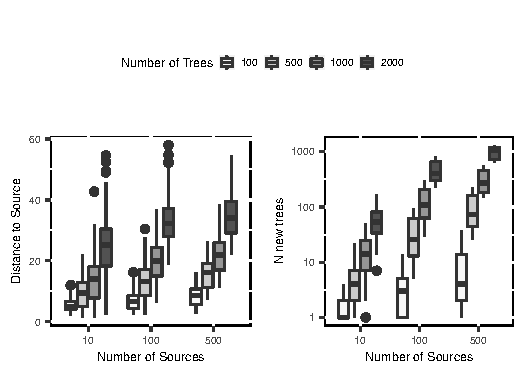
\includegraphics{Reeves_et_al_2021_Panda_ABM_files/figure-latex/figure-1-1.pdf}
\caption{\textbf{Left}: The effects of small scale tool use on the
distance \emph{Pounding Tools} move from their source. The box plots
show that the number of sources has a marginal effect on how far tools
move from their source. However, fig.width=3.5, message=FALSE,
warning=FALSE, paged.print=FALSE, the number of of Trees has positive
influence on how far tools can move. \textbf{Right}: The effect of small
scale tool use on the number of \emph{Trees} where tools use can occur.
Both the number of \emph{Sources} and \emph{Trees} has a positive
influence on the number of \emph{Trees} where tool use can occur. Note
that the Y axis for the right panel is in log scale \label{d2source}}
\end{figure}

One of the simplest and expected outcomes of the model is that small
scale tool use can occur when a \emph{Tree} and a \emph{Source} occur
within a 3 grid cell radius of each other. Tool use did not occur in 5\%
of the runs due to the fact that \emph{Trees} were never close enough to
a \emph{Source}. This was predominantly the case in model iterations
where both the number of \emph{Sources} and \emph{Trees} included in the
model were low (SOM: Table 1). Therefore simply increasing both the
number of \emph{Sources} or \emph{Trees} increases the number of places
and ultimately the likelihood that tool use can occur (SOM Figure 1:
left, ANOVA, F: 2435.41, P-value: 0).

When tool use does occur, 99\% of model iterations, led to movement of
\emph{Pounding Tools} across beyond the initial constraints of the
landscape. When a Pounding Tool is moved from a \emph{Source} to the
location of a \emph{Tree}, it becomes a secondary source of raw material
for other \emph{Trees} in the vicinity. Over time, provided that Trees
occur within a 3-grid cell radius of each other, the repeated transport
of \emph{Pounding Tools} incrementally moves Pounding Tools up to a
maximum distance of 58 grid cells from its \emph{Source}. The maximum
distance a \emph{Pounding Tool} can be moved is attenuated by the number
of \emph{Trees} in the model run. \emph{Pounding Tools} move greater
distances the number of \emph{Trees} is greater (Figure \ref{d2source},
left). In addition, the small nature of breakage fragments relative to
the size of the \emph{Pounding Tool} allows \emph{Pounding Tools} to be
used and transported 10s to 100s of times prior to total exhaustion
allowing tools of all qualities to be moved substantial distances from
their \emph{Sources} (SOM Table 2). Nevertheless, \emph{Pounding Tools}
of higher quality will move greater maximum distances from
\emph{Sources} prior to exhaustion. The size of the \emph{Pounding Tool}
also influences the maximum distance a pounding tool can be moved (SOM
Figure 2). This is because both of these variables influence the number
of times \emph{Pounding Tools} can be used and subsequently transported
(i.e.~use-life). This incremental transport of \emph{Pounding Tools}
away from their sources consequently increases the number of locations
where tool use can occur in 88\% of the runs (Figure \ref{d2source},
right). In other words, the repeated transport of tools across the
landscape increases the number of opportunities for tool-use on a given
landscape. The 12\% of Model runs that did not lead to an increased
access of Trees for nut-cracking are predominantly those where the
number of \emph{Trees} or \emph{Sources} are initially low (SOM Table
3).

Interestingly, the changing locations of \emph{Trees}, due to natural
growth and death cycles also strongly influences the above described
pattern. When holding the number of \emph{Sources}, and \emph{Trees}
constant, iterations where \emph{Trees} grow and die further increases
the number of trees that became available as loci for tool use (SOM
Figures 3, 4). When \emph{Tree} locations remains static (i.e.~they do
not die or grow), the number of \emph{Trees} that are accessible for
tool use events eventually plateaus thus limiting the area in which
\emph{Pounding Tools} can be redistributed (Figure \ref{tree_death},
left). In contrast. the accessibility of \emph{Trees} for tool use does
not diminish when Trees change locations over time instead, the number
of \emph{Trees} where tool use can occur continues to increase over time
(Figure \ref{tree_death}, right) in spite of the fact that
\emph{Pounding Tool} use and \emph{Tree} life cycle operate on different
temporal scales, the results show that the interaction of these
processes continuously increase the availability of the \emph{Trees}
across the landscape over time.

\begin{figure}
\centering
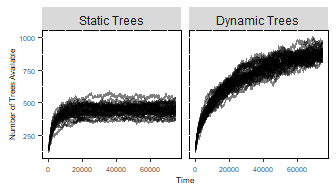
\includegraphics{Reeves_et_al_2021_Panda_ABM_files/figure-latex/figure-2-1.pdf}
\caption{The effect of tree death and growth and the number of trees
that come available due to the small scale transport of \emph{Pounding
Tools}. When \emph{trees} remain in a the same location (\textbf{Left})
the number of new trees that can be accessed due to the incremental
transport of \emph{Pounding Tools} raises and then eventually plateaus.
However, when \emph{Trees} die and grow (\textbf{Right}), these slow
changes in the locations of the trees further promotes the incidental
movement of \emph{Pounding Tools} away from their \emph{Sources}
\label{tree_death}}
\end{figure}

\hypertarget{material-signature}{%
\subsubsection{Material Signature}\label{material-signature}}

The spatial distribution, density and composition of the resulting
material record is dependent on the aspects of the landscape that
facilitate the movement of \emph{Pounding Tools} across space. When
\emph{Trees} are infrequent, the resulting assemblages form localized
patches in the grid-cells nearest to \emph{Sources} (Figure
\ref{distribution}, Top left). As small scale transport is able to move
\emph{Pounding Tools} move more freely as the number of Trees increases
the subsequent archaeological record becomes more widely spread (Figure
\ref{distribution}, Top Right). As a result, the growth and death of
\emph{Trees} has a substantial effect on the size and dispersion of the
archaeological record across space (Figure \ref{distribution}). Holding
the number of \emph{Trees} and the number \emph{Sources} constant, more
grids cells accumulate archaeological assemblages in model iterations
where \emph{Trees} grow and die in comparison with those where
\emph{Trees} do not change location. These results show that the
interaction between small scale tool transport and use with resource
distribution and longer term environmental change can substantially
influence the structure of the archaeological record.

\begin{figure*}

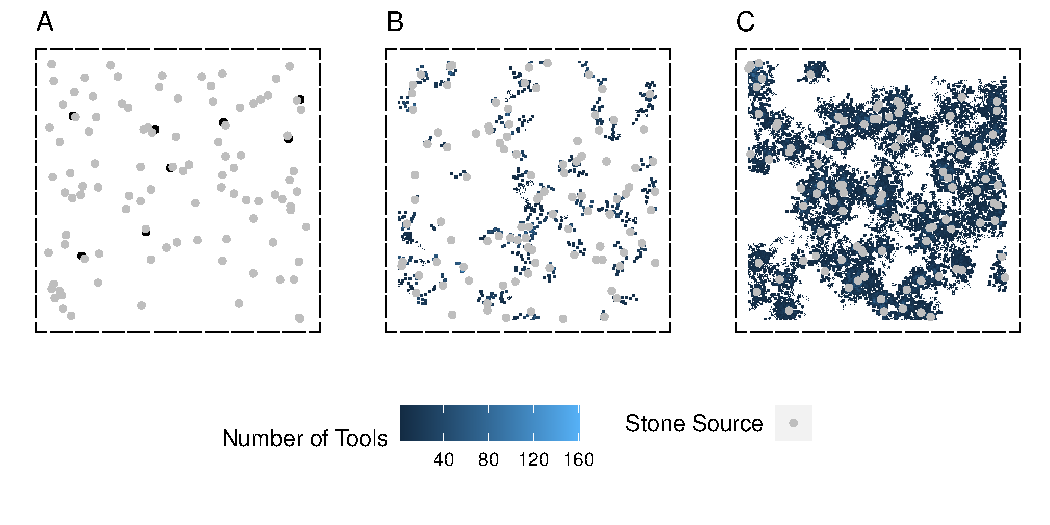
\includegraphics[width=6.5in]{Reeves_et_al_2021_Panda_ABM_files/figure-latex/figure 3-1.pdf}

\caption{A: The archaeological record when there are 100 sources and 100 trees. Notice that the subsequent archaeological record forms extremely localized patches of material. B: The archaeological record there 100 sources and 2000 trees. This archaeological record is becoming more wide-spread but remains localized. C: The archaeological record there 100 sources and 2000 trees where trees can die and regrow. The notice how the the growth and death of trees becomes substantially more widespread.}

\label{distribution}

\end{figure*}

In addition, the density of discarded material, as well as the size of
the \emph{Pounding Tools} are also structured across space. The amount
of discarded material per grid cell also forms a noisy distance-decay
relationship as the distance to the nearest source increases (Figure 4,
SOM Figure 5). The noise in the pattern is due to the fact that tool-use
and the location of trees are spatially auto-correlated. If trees occur
in such a way that allows \emph{Pounding Tools} to move from tree to
tree away from primary raw material sources, then a distance-decay
pattern will form. If, however, a single \emph{Tree} occurs in isolation
in proximity to a primary raw material source, then hammer-stones will
be used without being transported further than the location of the tree.
As a result, in model runs where the number of \emph{Trees} permit, the
repeated movement and use of \emph{Pounding Tools} results in a
distance--decay relationship where the range and average \emph{Pounding
Tool} size decreases as distance from its primary raw material source
increases (Figures 4, SOM Fig. 6, SOM Fig. 7).

Although \emph{Pounding Tools} are the only tool used within the model
they not are homogeneously distributed across the simulated landscape.
The number of \emph{Pounding Tools} within a given grid-cell also
follows a sharp distance-decay relationship with the nearest
\emph{Source}. In other words, \emph{Pounding tools} are found in there
highest quantities in assemblages nearest to \emph{Sources} and become
increasing scarce as the distance to the nearest \emph{Source}
increases. In fact, 78\% of the grid-cells that form material
assemblages are comprised entirely of fragments or exhausted Pounding
Tools. An additional 11\% of the grid-cells contain a single exhausted
\emph{Pounding Tool}.

\hypertarget{discussion}{%
\section{Discussion}\label{discussion}}

The results of our model elucidate the relationship tool-use involving
short term transport, between resource density (number of Sources and
Pounding Tools), environmental change, and the formation of the
archaeological record. While these results illustrate how the
distribution of resources within an environment ultimately constrains
the opportunities for tool-use, specific configurations of resources --
particularly those with large numbers of \emph{Trees} -- can have a long
lasting influence on the distribution of materials needed for tool use.
The model also shows how short term instances of tool transportation can
lead to the movement of \emph{Pounding Tools} across long distances over
time thus increasing the number of opportunities for tool use. This long
term modification of the landscape is further encouraged by the
widespread distribution of foraging opportunities to use tools (in our
model \emph{Trees}). These dynamics not only influence the prevalence of
locations where it is possible to forage where tools are necessary but
also the structure of the resulting archaeological record.

\begin{figure*}

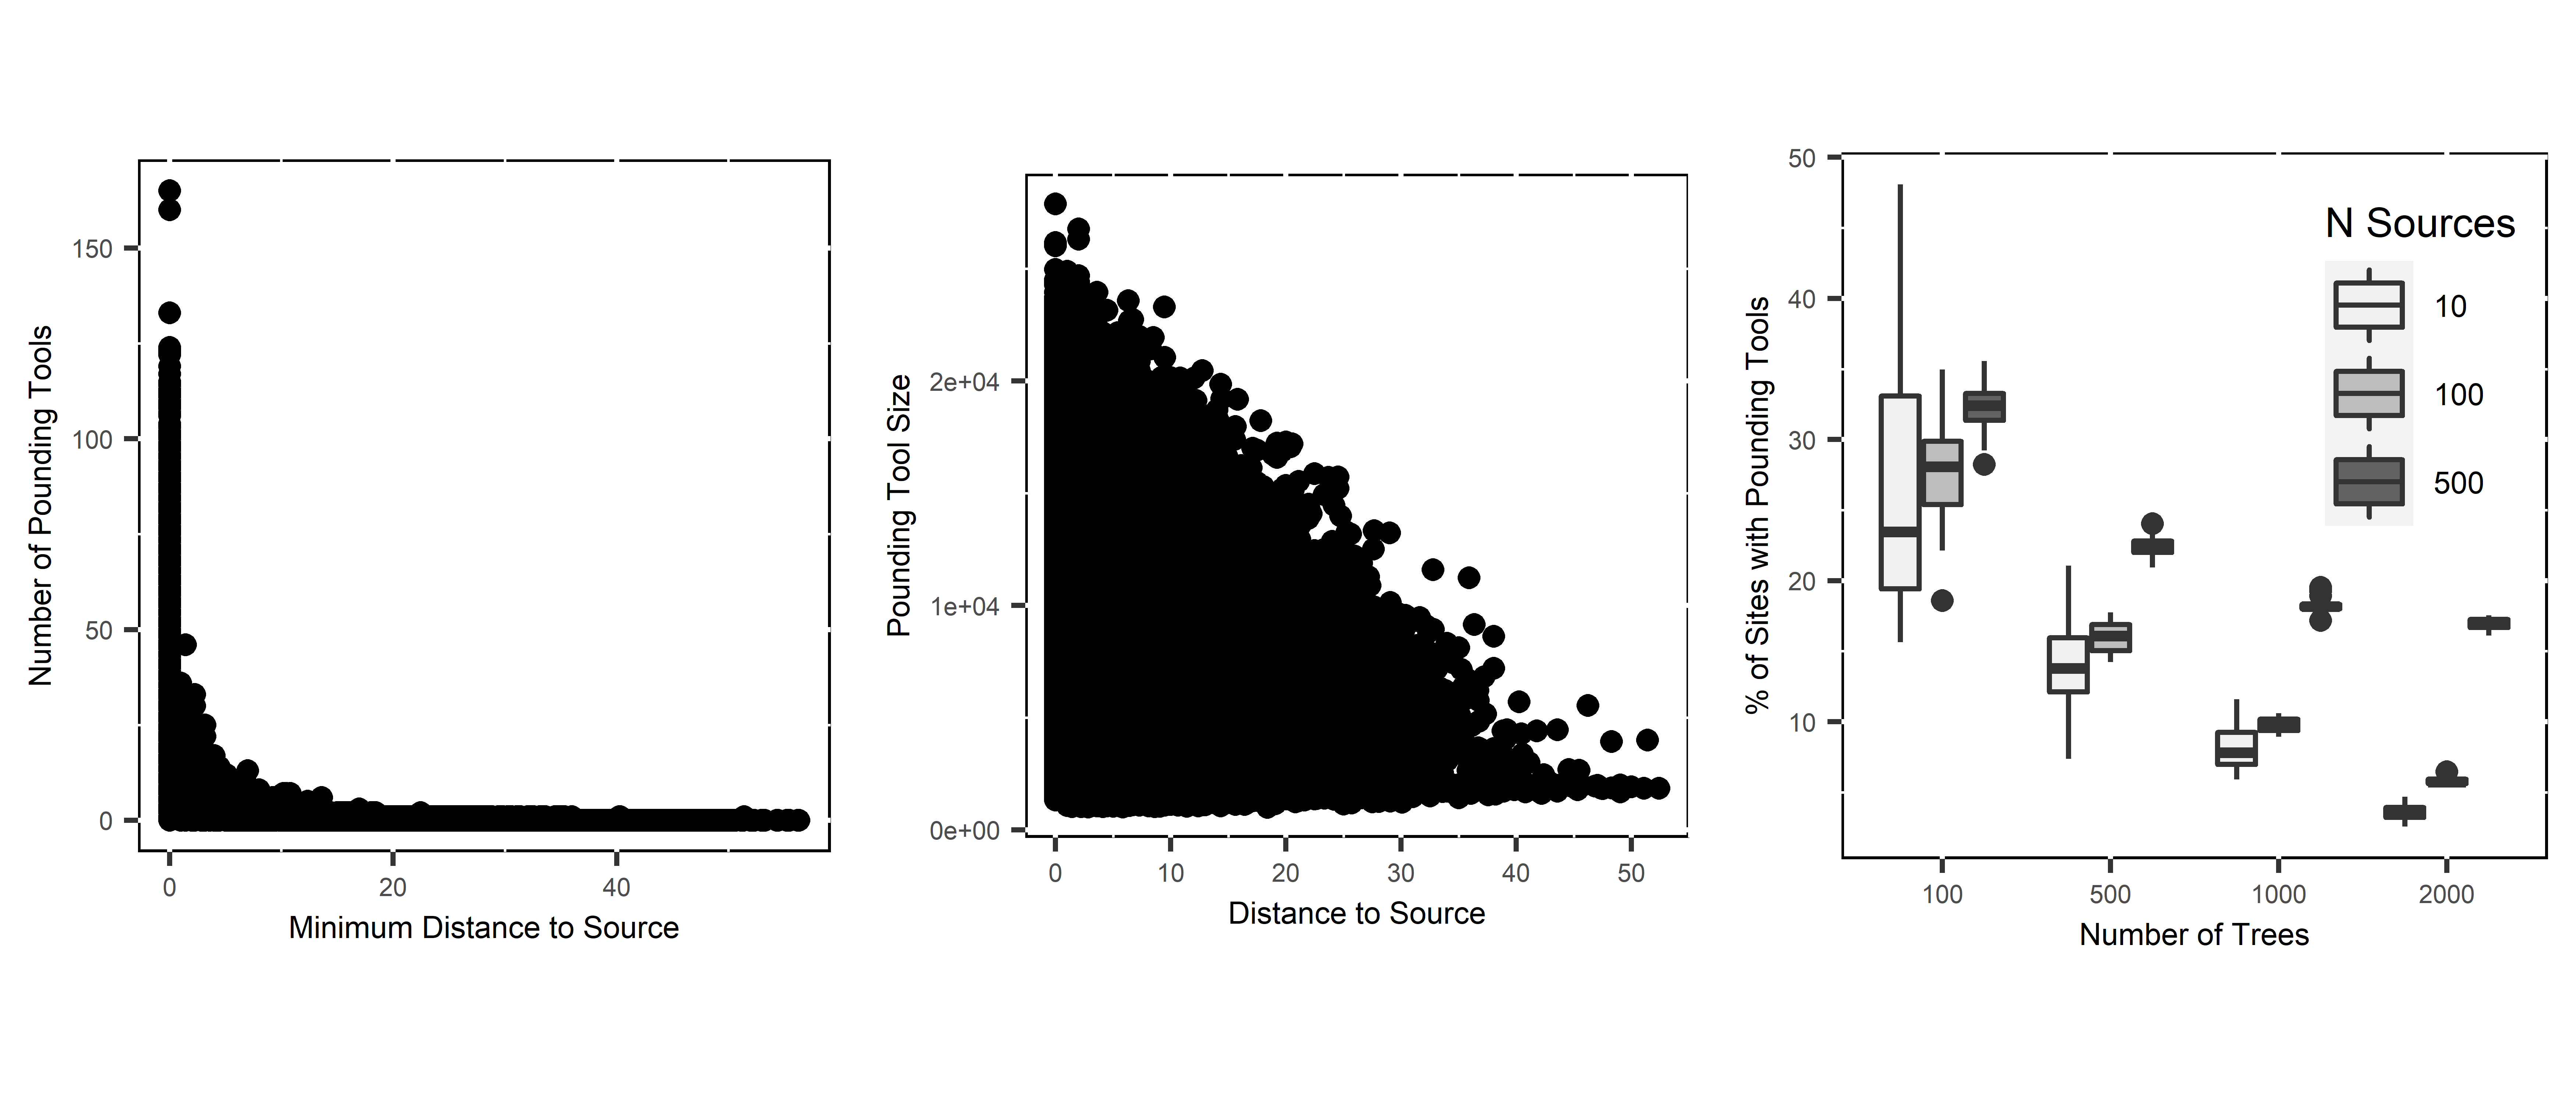
\includegraphics[width=6.5in]{Reeves_et_al_2021_Panda_ABM_files/figure-latex/figure 4-1.pdf}

\caption{Left: A scatter plot showing the relationship between the number of artifacts (e.g. Pounding Tools and fragments) present within a grid-cell and its distance to the nearest source. Grid-cells closer to sources can possess a wider range of artifacts, whereas grid-cells farther from the source consistently possess few artifacts. Middle: Scatter plot showing the relationship of the number Pounding Tools in a grid cell with the distance to the nearest source. Right: The relationship between Pounding Tool size and distance to its source. Note: All plots show runs where the number of sources is 100 and the number of trees is 2000. See SOM figures 5, 6, and for other model runs.}

\label{assemblages}

\end{figure*}

\hypertarget{environmental-facilitators-of-tool-use}{%
\subsubsection{Environmental Facilitators of Tool
Use}\label{environmental-facilitators-of-tool-use}}

It has often been argued that patterns of tool assisted foraging are
driven by encounter rates with resources requiring and raw material
needed for tool use (37, 38). The results of our model provide further
support for this hypothesis by showing that when tool-using behavior is
expedient, the number of opportunities use tools is entirely regulated
by the frequency and co-occurrence of resources and sources of material
in space. Nevertheless, when there are certain configurations of
resources, even short bouts of transport can have long term effects on
the spatial distribution tool materials and the number of opportunities
for tool use beyond what the structure of the landscape naturally
allows. In these situations, opportunities for tool-use are not limited
by the constraints of the environment and can even be increased by the
tool using behavior itself. This work shows that even small scale tool
using behaviors have the capacity to modify the availability of a
resource through the redistribution tool material. In this light, the
model illustrates the niche constructing capacity of such small scale
tool using behaviors as increasing the availability of tool-facilitated
resources also increases number of times an individual encounters tool
using opportunities.

\hspace{0pt} In addition, the model demonstrates how these small scale
tool using behaviors generate positive feedback with the changes in
tool-use locations that further enhances the availability of resources
and the number of tool using opportunities over the long term. Moreover,
the fact that the model Though environmental dynamics are often argued
to influence behavioral patterns across evolutionary time-scales but,
such arguments lack mechanisms that causally link the two processes
together (16, 39, 40). Our model contributes to this discussion by
illustrating how processes that operate on different temporal scales
produces feedback. While the model does not consider reproduction, these
results may imply that new generations of a population where such
feedback is in effect inherit a landscape in which resources associated
with this type of tool using behavior are more accessible than they were
in previous generations.

\hypertarget{implications-for-chimpanzee-stone-tool-use}{%
\subsubsection{Implications for Chimpanzee Stone Tool
Use}\label{implications-for-chimpanzee-stone-tool-use}}

Although stone tool use among \emph{Pan} is considered to be highly
constrained by the environment (10), the results of the model imply
Chimpanzees have to capacity to modify their environments in a way that
may have a lasting effect the landscape that is inherited by future
generations of Chimpanzees. Nut-cracking hammerstones are recorded up to
2 kilometers from the nearest naturally occurring source of stone in the
Tai Forest. Moreover, these hammers have been shown follow a
distance-decay pattern where hammers are smaller are more utilized the
farther they are found from the nearest source (18). This spatial
patterning is consistent with the results of the model and may such
suggest that the Chimpanzees of the Tai Forest may be modifying
distribution of tool using materials. Although tool transport and use
within the model is hard-coded into the agent's behavior within our
model, tool use, within chimpanzee populations, has previously been
described as a socially learned behavior (12, 41, 42). As such, the
results of our model within the context of chimpanzee behavior suggest
that chimpanzees may unintentionally modify their accessibility to
resources through a culturally learned behavior. Increasing the number
of opportunities for tool use also increases the number of social
opportunities for learning and the transmission of tool using skills
(38). In this sense, the results of our model shows how short term bouts
of transport also may reinforce the prevalence of tool use within
chimpanzee populations by causing future generations to inherit a
landscape in which the number of tool-use opportunities is greater than
if was before.

However, unlike the model percussive tools do not accumulate at tool-use
sites nearest to sources but rather remain infrequent across the
landscape. This maybe related to a combination of the minimum distance
of nut-trees to a source of stone and transport costs or even an
additional bias to re-use tools as opposed acquiring new material from a
source. This difference between the model and nut-cracking in the Tai
Forest, may highlight the delicate balance between the environment,
availability of tool using resources, and behavior, that attenuates the
spatial-temporal impact of small scale tool using behaviors on the
landscape.

\hypertarget{implications-for-hominin-evolution}{%
\subsubsection{Implications for hominin
evolution}\label{implications-for-hominin-evolution}}

\hspace{0pt} One of the hallmarks of hominin and human niche is the
capacity to enable to increase their access to resources through the
transport and reuse of tool material (23, 43--45). The relocation of
such materials into material poor areas, effectively makes a lasting
change to the environment which, in turn conditions, the mobility,
foraging, or even settlement strategies of future generations (6,
46--48). Within this context, our model shows that even transport over
short distances can modify landscapes in such a way that increases, both
the opportunities for tool use and the accessibility of resources.

\begin{verbatim}
It may be that such interactions between the distribution of resources and short term tool transport behavior had the capacity to generate feedback that may have influenced the role tool use in  hominin evolution. For example, percussive tools may facilitated access to animal protein through the breakage bones prior to the emergence core and flake technology [@thompsonOriginsHumanPredatory2019]. Within the context of the model it is plausible, that the interaction between short distance transport of percussive tools and the changing locations of animal carcasses as the result of the emergence of new kills and the decomposition of old kills, would have created a dynamic that would systematically seed a lake margin environment with percussive tools. This would increase both the number of opportunities and encounter rates with scavengable carcasses and in turn increase the contribution of animal protein to the hominin diet. Such encounter rates would have been critical to recognizing animal carcasses as a food resource and its increased consumption over time [@thompsonOriginsHumanPredatory2019]. In may that simple interactions between local environmental dynamics and tool transport may have contributed to the increased consumption of protein which is argued to have played an important role in hominin brain evolution and even the emergence of _H. erectus_ [@antonEvolutionEarlyHomo2014; @lalandNicheConstructionBiological2000; @pattersonComparativeIsotopicEvidence2019].
\end{verbatim}

\hypertarget{implications-for-the-archaeological-record}{%
\subsubsection{Implications for the archaeological
record}\label{implications-for-the-archaeological-record}}

In order to understand if the processes illustrated in the model had
bearing on the past, evidence of such dynamics must gleaned from a
static material record. As such, the results of the model provides novel
insights into the transformation of these processes into an
archaeological record. Percussive tools are the most characteristic
artefact of the primate stone tool record and are well described in both
human and nonhuman primates (49, 50). The results of the model
illustrate how the tangible traces on left on percussive tools in terms
of their degree of utilization and their distance from their source
location are result of this interaction between external and behavioral
processes. Both of these attributes can be inferred from archaeological
contexts (18, 51).

However, documenting this pattern in an archaeological context is far
more complex. While the results of this study show that in some
circumstances, primate percussive behavior can produce a wide spread
material record the ubiquity of pounding tools across the landscape is
not homogenous. The percussive tools only occur in large quantities in
assemblages where stone is readily available (i.e.~close to Sources) and
are relatively scarce or even absent in areas more distant from sources.
In these distant places suitable pounding tools less available and
therefore more likely to be transported more often. If there is a need
to continuously transport and utilize the same hammerstones, as is
observed in the model, then there may be little opportunity for tools to
enter the archaeological record whole. Such tools may only enter the
archaeological record as fragments or as an exhausted tool, at which
point, they become almost archaeologically invisible (32). This
phenomenon is echoed in the Tai Forest, for example, stone tool use was
continuously observed from 1979 to 1983 site of Panda 100, until the
death of the tree in 1984 (52). Yet, archaeological investigation of the
site yielded little to no evidence of complete hammerstones, suggesting
that the discarded hammer stones at the once live tree become a
secondary source of material for other nut bearing trees (34, 53).

Although there is currently no physical evidence, it has been postulated
that a culture of percussive technology similar to that of modern-day
chimpanzees may have existed prior to the earliest known archaeological
evidence of early hominins (10, 13, 54). Few expectations have, however,
been set forth regarding the composition of this archaeological record.
Here we build upon the expectations of Panger et al. (15) by
illustrating how the structure of the environment influences structure
of the archaeological record. The results of this model suggest that the
associated record may range from a few localized patches to a widespread
distribution of archaeological sites throughout the landscape. If the
earliest durable evidence of hominin tool-use is manifested as
percussive tools then this record may be difficult to recover. While the
model does show that this behavior can lead to the aggregation of large
quantities of percussive tools, it also suggests that such localities
are rare. In other environmental circumstances the archaeological record
is far more wide spread, but most assemblages would be comprised of
mostly fragments. Such a record, even if widespread, would be difficult
to recognize as early forms of tool use let alone distinguish from
non-anthropogenic processes.

\hypertarget{conclusion}{%
\section{Conclusion}\label{conclusion}}

Though small scale tool-use is ultimately constrained by its
environment. This model shows that hammerstone transport over time can
have a significant effect on the facilitation of tool behavior itself.
The aggregate effect of short transportation events can improve the
accessibility of resources within a landscape over time. This landscape
pattern of unintentional tool provisioning not only potentially
mitigates against local changes in the availability of resources but
also increases the opportunity for nut cracking to be carried out. In
this sense this tool-using behavior provides chimpanzees and potentially
other tool-using non-human primates the capacity to positively modify
their environments.. In the context of living Chimpanzee populations,
the results of the model in combination with ethological data have the
potential to incrementally modify their environments through a
culturally learned behaviors.

\showmatmethods
\showacknow
\pnasbreak

\hypertarget{refs}{}
\begin{CSLReferences}{0}{0}
\leavevmode\hypertarget{ref-hillEmergenceHumanUniqueness2009}{}%
\CSLLeftMargin{1. }
\CSLRightInline{Hill K, Barton M, Magdalena Hurtado A (2009) The
emergence of human uniqueness: {Characters} underlying behavioral
modernity. \emph{Evolutionary Anthropology} 18(5):187--200.}

\leavevmode\hypertarget{ref-boydNotGenesAlone2005}{}%
\CSLLeftMargin{2. }
\CSLRightInline{Boyd R, Richardson PJ (2005) \emph{Not by {Genes Alone}:
{How Culture Transformed Human Evolution}} ({University of Chicago
Press}, {Chicago}).}

\leavevmode\hypertarget{ref-danchinDNAIntegratingInclusive2011}{}%
\CSLLeftMargin{3. }
\CSLRightInline{Danchin Ã, et al. (2011) Beyond {DNA}: Integrating
inclusive inheritance into an extended theory of evolution. \emph{Nat
Rev Genet} 12(7):475--486.}

\leavevmode\hypertarget{ref-fogartyNicheConstructionCultural2017}{}%
\CSLLeftMargin{4. }
\CSLRightInline{Fogarty L, Creanza N (2017) The niche construction of
cultural complexity: Interactions between innovations, population size
and the environment. \emph{Philosophical Transactions of the Royal
Society B: Biological Sciences} 372(1735):20160428.}

\leavevmode\hypertarget{ref-lalandCulturalNicheConstruction2011}{}%
\CSLLeftMargin{5. }
\CSLRightInline{Laland KN, OÃâNANANAâNABri MJ (2011) Cultural {Niche
Construction}: {An Introduction}. \emph{Biol Theory} 6(3):191--202.}

\leavevmode\hypertarget{ref-lalandNicheConstructionBiological2000}{}%
\CSLLeftMargin{6. }
\CSLRightInline{Laland KN, Odling-Smee J, Feldman MW (2000) Niche
construction, biological evolution, and cultural change.
\emph{Behavioral and Brain Sciences} 23(1):131--146.}

\leavevmode\hypertarget{ref-obrienDualInheritanceCultural2017}{}%
\CSLLeftMargin{7. }
\CSLRightInline{O'Brien MJ, Bentley RA (2017) Dual {Inheritance},
{Cultural Transmission}, and {Niche Construction}. \emph{The {Handbook}
of {Culture} and {Biology}}, eds Causadias JM, Telzer EH, Gonzales NA
({John Wiley \& Sons, Inc.}, {Hoboken, NJ, USA}), pp 179--201.}

\leavevmode\hypertarget{ref-odling-smeeNicheConstructionTheory2013}{}%
\CSLLeftMargin{8. }
\CSLRightInline{Odling-Smee J, Erwin DH, Palkovacs EP, Feldman MW,
Laland KN (2013) Niche {Construction Theory}: {A Practical Guide} for
{Ecologists}. \emph{The Quarterly Review of Biology} 88(1):3--28.}

\leavevmode\hypertarget{ref-rendellRunawayCulturalNiche2011}{}%
\CSLLeftMargin{9. }
\CSLRightInline{Rendell L, Fogarty L, Laland KN (2011) Runaway cultural
niche construction. \emph{Philosophical Transactions of the Royal
Society B: Biological Sciences} 366(1566):823--835.}

\leavevmode\hypertarget{ref-carvalhoToolcompositeReuseWild2009}{}%
\CSLLeftMargin{10. }
\CSLRightInline{Carvalho S, Biro D, McGrew WC, Matsuzawa T (2009)
Tool-composite reuse in wild chimpanzees ({Pan} troglodytes):
Archaeologically invisible steps in the technological evolution of early
hominins? \emph{Anim Cogn} 12(1):103--114.}

\leavevmode\hypertarget{ref-lalandAnimalCultures2008}{}%
\CSLLeftMargin{11. }
\CSLRightInline{Laland K (2008) Animal {Cultures}. \emph{Current
biology} 18(9):366--370.}

\leavevmode\hypertarget{ref-lunczPrimateArchaeologyReveals2015}{}%
\CSLLeftMargin{12. }
\CSLRightInline{Luncz LV, Wittig RM, Boesch C (2015) Primate archaeology
reveals cultural transmission in wild chimpanzees ({Pan} troglodytes
verus). \emph{Philos Trans R Soc Lond B Biol Sci} 370(1682).
doi:\href{https://doi.org/10.1098/rstb.2014.0348}{10.1098/rstb.2014.0348}.}

\leavevmode\hypertarget{ref-mcgrewChimpanzeeMaterialCulture1992}{}%
\CSLLeftMargin{13. }
\CSLRightInline{McGrew W (1992) \emph{Chimpanzee {Material Culture}:
{Implications} for {Human Evolution}} ({Cambridge University Press},
{Cambridge}).}

\leavevmode\hypertarget{ref-sanzEcologicalSocialCorrelates2013}{}%
\CSLLeftMargin{14. }
\CSLRightInline{Sanz CM, Morgan DB (2013) Ecological and social
correlates of chimpanzee tool use. \emph{Philosophical Transactions of
the Royal Society B: Biological Sciences} 368(1630):20120416.}

\leavevmode\hypertarget{ref-pangerOlderOldowanRethinking2003}{}%
\CSLLeftMargin{15. }
\CSLRightInline{Panger MA, Brooks AS, Richmond BG, Wood B (2003) Older
than the {Oldowan}? {Rethinking} the emergence of hominin tool use.
\emph{Evolutionary Anthropology: Issues, News, and Reviews}
11(6):235--245.}

\leavevmode\hypertarget{ref-stinerChallengesDocumentingCoevolution2020}{}%
\CSLLeftMargin{16. }
\CSLRightInline{Stiner MC (2020) The challenges of documenting
coevolution and niche construction: {The} example of domestic spaces.
\emph{Evolutionary Anthropology}:evan.21878.}

\leavevmode\hypertarget{ref-boeschMentalMapWild1984}{}%
\CSLLeftMargin{17. }
\CSLRightInline{Boesch C, Boesch H (1984) Mental map in wild
chimpanzees: {An} analysis of hammer transports for nut cracking.
\emph{Primates} 25(2):160--170.}

\leavevmode\hypertarget{ref-lunczDistancedecayEffectStone2016}{}%
\CSLLeftMargin{18. }
\CSLRightInline{Luncz LV, Proffitt T, Kulik L, Haslam M, Wittig RM
(2016) Distance-decay effect in stone tool transport by wild
chimpanzees. \emph{Proceedings of the Royal Society B: Biological
Sciences} 283(1845):20161607.}

\leavevmode\hypertarget{ref-gifford-gonzalezBonesAreNot1991}{}%
\CSLLeftMargin{19. }
\CSLRightInline{Gifford-Gonzalez D (1991) Bones are not enough:
{Analogues}, knowledge, and interpretive strategies in zooarchaeology.
\emph{Journal of Anthropological Archaeology} 10(3):215--254.}

\leavevmode\hypertarget{ref-perreaultQualityArchaeologicalRecord2019}{}%
\CSLLeftMargin{20. }
\CSLRightInline{Perreault C (2019) \emph{The {Quality} of the
{Archaeological Record}} ({University of Chicago Press}, {Chicago})
Available at:
\url{https://www.press.uchicago.edu/ucp/books/book/chicago/Q/bo39582137.html}
{[}Accessed September 13, 2019{]}.}

\leavevmode\hypertarget{ref-baileyTimePerspectivesPalimpsests2007}{}%
\CSLLeftMargin{21. }
\CSLRightInline{Bailey G (2007) Time perspectives, palimpsests and the
archaeology of time. \emph{Journal of Anthropological Archaeology}
26(2):198--223.}

\leavevmode\hypertarget{ref-brooksPreservationActivityAreas1987}{}%
\CSLLeftMargin{22. }
\CSLRightInline{Brooks AS, Yellen JE (1987) The {Preservation} of
{Activity Areas} in the {Archaeological Record}: {Ethnoarchaeological}
and {Archaeological Work} in {NOrthwest Ngamiland}, {Botswana}.
\emph{Methog and {Theory} for {Activity Area Research}: {An
Ethnoarchaeological Approach}} ({Columbia University Press}, {New
York}), pp 63--106.}

\leavevmode\hypertarget{ref-schickModelingFormationEarly1987}{}%
\CSLLeftMargin{23. }
\CSLRightInline{Schick KD (1987) Modeling the formation of {Early Stone
Age} artifact concentrations. \emph{Journal of Human Evolution}
16(7-8):789--807.}

\leavevmode\hypertarget{ref-Stern1993}{}%
\CSLLeftMargin{24. }
\CSLRightInline{Stern N, et al. (1993) The {Structure} of the {Lower
Pleistocene Archaeological Record}: {A Case Study From} the {Koobi Fora
Formation} {[}and {Comments} and {Reply}{]}. \emph{Current Anthropology}
34(3):201--225.}

\leavevmode\hypertarget{ref-sternImplicationsTimeaveragingReconstructing1994}{}%
\CSLLeftMargin{25. }
\CSLRightInline{Stern N (1994) The implications of time-averaging for
reconstructing the land-use patterns of early tool-using hominids.
\emph{Journal of Human Evolution} 27(1-3):89--105.}

\leavevmode\hypertarget{ref-rezekAggregatesFormationalEmergence2020}{}%
\CSLLeftMargin{26. }
\CSLRightInline{Rezek Z, et al. (2020) Aggregates, {Formational
Emergence}, and the {Focus} on {Practice} in {Stone Artifact
Archaeology}. \emph{J Archaeol Method Theory}.
doi:\href{https://doi.org/10.1007/s10816-020-09445-y}{10.1007/s10816-020-09445-y}.}

\leavevmode\hypertarget{ref-schellingMicromotivesMacrobehaviors1978}{}%
\CSLLeftMargin{27. }
\CSLRightInline{Schelling TC (1978) \emph{Micromotives and
{Macrobehaviors}} ({W. W. Norton \& Company}, {Toronto})
doi:\href{https://doi.org/10.2307/2989930}{10.2307/2989930}.}

\leavevmode\hypertarget{ref-davidsonFinishedArtefactFallacy2002}{}%
\CSLLeftMargin{28. }
\CSLRightInline{Davidson I (2002) The {Finished Artefact Fallacy}:
{Acheulean Hand}-axes and {Language Origins} ({Oxford University
Press}). Available at:
\url{https://rune.une.edu.au/web/handle/1959.11/1837} {[}Accessed
February 22, 2021{]}.}

\leavevmode\hypertarget{ref-daviesModellingPalimpsestExploratory2016}{}%
\CSLLeftMargin{29. }
\CSLRightInline{Davies B, Holdaway SJ, Fanning PC (2016) Modelling the
palimpsest: {An} exploratory agent-based model of surface archaeological
deposit formation in a fluvial arid {Australian} landscape.
\emph{Holocene} 26(3):450--463.}

\leavevmode\hypertarget{ref-dibbleMajorFallaciesSurrounding2017}{}%
\CSLLeftMargin{30. }
\CSLRightInline{Dibble HL, et al. (2017) Major {Fallacies Surrounding
Stone Artifacts} and {Assemblages}. \emph{Journal of Archaeological
Method and Theory} 24.
doi:\href{https://doi.org/10.1007/s10816-016-9297-8}{10.1007/s10816-016-9297-8}.}

\leavevmode\hypertarget{ref-frisonFunctionalAnalysisCertain1968}{}%
\CSLLeftMargin{31. }
\CSLRightInline{Frison GC (1968) A {Functional Analysis} of {Certain
Chipped Stone Tools}. \emph{American Antiquity} 33(2):149--155.}

\leavevmode\hypertarget{ref-schifferFormationProcessesArchaeological1987}{}%
\CSLLeftMargin{32. }
\CSLRightInline{Schiffer MB (1987) \emph{Formation processes of the
archaeological record} ({University of New Mexico Press}) Available at:
\url{https://books.google.co.ke/books/about/Formation_processes_of_the_archaeologica.html?id=TMpVlJ8zK78C\&redir_esc=y}.}

\leavevmode\hypertarget{ref-shottLowerPaleolithicIndustries2008}{}%
\CSLLeftMargin{33. }
\CSLRightInline{Shott MJ (2008) Lower {Paleolithic Industries}, {Time},
and the {Meaning} of {Assemblage Variation}. \emph{Time in
{Archaeology}}, eds Holdaway SJ, Wandsnider L ({University of Utah
Press}, {Salt Lake City}), pp 46--50.}

\leavevmode\hypertarget{ref-proffittRevisitingPanda1002018}{}%
\CSLLeftMargin{34. }
\CSLRightInline{Proffitt T, Haslam M, Mercader JF, Boesch C, Luncz LV
(2018) Revisiting {Panda} 100, the first archaeological chimpanzee
nut-cracking site. \emph{Journal of Human Evolution} 124:117--139.}

\leavevmode\hypertarget{ref-masadMESAAgentBasedModeling2015}{}%
\CSLLeftMargin{35. }
\CSLRightInline{Masad D, Kazil J (2015) {MESA}: {An Agent}-{Based
Modeling Framework}. \emph{Proceedings of the 14th Python in Science
Conference (SCIPY 2015)}:53--60.}

\leavevmode\hypertarget{ref-rossum1995python}{}%
\CSLLeftMargin{36. }
\CSLRightInline{van Rossum G (1995) Python tutorial, technical report
{CS}-{R9526}. \emph{Centrum voor Wiskunde en Informatica (CWI),
Amsterdam}.}

\leavevmode\hypertarget{ref-foxIntelligentToolUse1999}{}%
\CSLLeftMargin{37. }
\CSLRightInline{Fox EA, Sitompul AF, Van Schaik CP (1999) Intelligent
tool use in wild {Sumatran} orangutans. \emph{The mentality of gorillas
and orangutans} 480:99--116.}

\leavevmode\hypertarget{ref-koopsEcologyCultureEnvironmental2013}{}%
\CSLLeftMargin{38. }
\CSLRightInline{Koops K, McGrew WC, Matsuzawa T (2013) Ecology of
culture: Do environmental factors influence foraging tool use in wild
chimpanzees, {Pan} troglodytes verus? \emph{Animal Behaviour}
85(1):175--185.}

\leavevmode\hypertarget{ref-behrensmeyerClimateChangeHuman2006}{}%
\CSLLeftMargin{39. }
\CSLRightInline{Behrensmeyer AK (2006) Climate {Change} and {Human
Evolution}. \emph{Science} 311(5760):476--478.}

\leavevmode\hypertarget{ref-kingstonShiftingAdaptiveLandscapes2007}{}%
\CSLLeftMargin{40. }
\CSLRightInline{Kingston JD (2007) Shifting {Adaptive Landscapes}:
{Progress} and {Challenges} in {Reconstructing Early Hominid
Environments}. \emph{Yearbook of Physical Anthropology} 50:20--58.}

\leavevmode\hypertarget{ref-whitenCulturalPanthropology2003}{}%
\CSLLeftMargin{41. }
\CSLRightInline{Whiten A, Horner V, Marshall-Pescini S (2003) Cultural
panthropology. \emph{Evol Anthropol} 12(2):92--105.}

\leavevmode\hypertarget{ref-whitenCulturesChimpanzees1999}{}%
\CSLLeftMargin{42. }
\CSLRightInline{Whiten A, et al. (1999) Cultures in chimpanzees.
\emph{Nature} 399(6737):682--685.}

\leavevmode\hypertarget{ref-binfordWillowSmokeDogs1980}{}%
\CSLLeftMargin{43. }
\CSLRightInline{Binford LR (1980) Willow {Smoke} and {Dogs} ' {Tails} :
{Hunter}-{Gatherer Settlement Systems} and {Archaeological Site
Formation}. \emph{American Antiquity} 45(1):4--20.}

\leavevmode\hypertarget{ref-kuhnMousterianLithicTechnology1995}{}%
\CSLLeftMargin{44. }
\CSLRightInline{Kuhn SL (1995) \emph{Mousterian {Lithic Technology}: {An
Ecological Perspective}} ({Princeton University Press}) Available at:
\url{http://books.google.com?id=RUkABAAAQBAJ}.}

\leavevmode\hypertarget{ref-pottsWhyOldowanPlioPleistocene1991}{}%
\CSLLeftMargin{45. }
\CSLRightInline{Potts R (1991) Why the {Oldowan}? {Plio}-{Pleistocene
Toolmaking} and the {Transport} of {Resources}. \emph{Journal of
Anthropological Research} 47(2):153--176.}

\leavevmode\hypertarget{ref-braunEcosystemEngineeringQuaternary2020}{}%
\CSLLeftMargin{46. }
\CSLRightInline{Braun DR, et al. (2020) Ecosystem engineering in the
{Quaternary} of the {West Coast} of {South Africa}. \emph{Evolutionary
Anthropology: Issues, News, and Reviews} n/a(n/a).
doi:\href{https://doi.org/10.1002/evan.21886}{10.1002/evan.21886}.}

\leavevmode\hypertarget{ref-haasForagerMobilityConstructed2019}{}%
\CSLLeftMargin{47. }
\CSLRightInline{Haas R, Kuhn SL (2019) Forager {Mobility} in
{Constructed Environments}. \emph{Current Anthropology} 60(4):499--535.}

\leavevmode\hypertarget{ref-iovitaOperationalizingNicheConstruction2021}{}%
\CSLLeftMargin{48. }
\CSLRightInline{Iovita R, et al. (2021) Operationalizing niche
construction theory with stone tools. \emph{Evolutionary
Anthropology}:evan.21881.}

\leavevmode\hypertarget{ref-arroyoPoundingToolsHWK2018}{}%
\CSLLeftMargin{49. }
\CSLRightInline{Arroyo A, de la Torre I (2018) Pounding tools in {HWK
EE} and {EF}-{HR} ({Olduvai Gorge}, {Tanzania}): {Percussive} activities
in the {Oldowan}-{Acheulean} transition. \emph{Journal of Human
Evolution} 120:402--421.}

\leavevmode\hypertarget{ref-benito-calvoFirstGISAnalysis2015}{}%
\CSLLeftMargin{50. }
\CSLRightInline{Benito-Calvo A, Carvalho S, Arroyo A, Matsuzawa T, de la
Torre I (2015) First {GIS Analysis} of {Modern Stone Tools Used} by
{Wild Chimpanzees} ({Pan} troglodytes verus) in {Bossou}, {Guinea},
{West Africa}. \emph{PLoS ONE} 10(3):e0121613.}

\leavevmode\hypertarget{ref-lathamNondestructiveXrfCharacterization1992}{}%
\CSLLeftMargin{51. }
\CSLRightInline{Latham TS, Sutton PA, Verosub KL (1992) Non-destructive
xrf characterization of basaltic artifacts from {Truckee}, {California}.
\emph{Geoarchaeology} 7(2):81--101.}

\leavevmode\hypertarget{ref-boeschWildCulturesComparison2014}{}%
\CSLLeftMargin{52. }
\CSLRightInline{Boesch C (2014) \emph{Wild cultures a comparison between
chimpanzee and human cultures.} ({Cambridge University Press},
{Cambridge}).}

\leavevmode\hypertarget{ref-mercaderExcavationChimpanzeeStone2002}{}%
\CSLLeftMargin{53. }
\CSLRightInline{Mercader J, Panger M, Boesch C (2002) Excavation of a
{Chimpanzee Stone Tool Site} in the {African Rainforest}. \emph{Science}
296(5572):1452--1455.}

\leavevmode\hypertarget{ref-mcgrewSearchLastCommon2010}{}%
\CSLLeftMargin{54. }
\CSLRightInline{McGrew WC (2010) In search of the last common ancestor:
New findings on wild chimpanzees. \emph{Philosophical Transactions of
the Royal Society B: Biological Sciences} 365(1556):3267--3276.}

\end{CSLReferences}



% Bibliography
% \bibliography{pnas-sample}

\end{document}
